\documentclass[11pt]{article}
% \usepackage[utf8]{inputenc}
% \usepackage{amsfonts}
\usepackage{cs282}
\usepackage{markup}
\usepackage{macros}
\usepackage{amsmath}
\usepackage{graphicx} %for includegraphics
\usepackage{float}
\usepackage{algorithm} % for algorithm environment
\usepackage[symbol]{footmisc}
\renewcommand{\thefootnote}{\fnsymbol{footnote}}

% Toggle comment between the following two lines to see/hide solutions
\newcommand{\sol}[1]{{\vspace{2pt} \color{blue} \textbf{Solution: } #1}} % solutions in blue
%\newcommand{\sol}[1]{} % no solution sketches

\def\title{Final Project Problem Set}
\date{Fall 2022}

\begin{document}

\maketitle


\begin{qunlist}
    % Include any questions here with \input{}
    \qns{Weight Decoupling, Adaptive Methods, and Finally, AdamW \cite{Loshchilov}}


\href{https://pytorch.org/docs/stable/generated/torch.optim.AdamW.html}{AdamW}, by definition, is an weight-decoupled adaptive stochastic optimization method that implements weight decaying effects onto Adam (ADAptive Moment estimation) through entering in coresponding values for the \texttt{weight\_decay} argument. But if you take a look at PyTorch's documentation on \href{https://pytorch.org/docs/stable/generated/torch.optim.Adam.html}{Adam}, we also see a \texttt{weight\_decay} parameter for us to set - which makes one wonder, "setting this parameter for Adam should be equivalent to doing the same with AdamW - right?". In this problem, we will explore how these two methods are not equivalent and how \texttt{weight\_decay} in Adam is a potential misnomer as $\ell_2$-regularization $\neq$ weight decay in Adam. Along the way, we'll also introduce you to the idea of weight decoupling, fundamentals of adaptive gradient methods, and its relationship with $\ell_2$-regularization and weight decay. Finally, we will convince you that AdamW, a weight decoupled version of Adam, leads to a hyperparameter space that is better behaved and easier to tune.

\begin{enumerate}[(a)]
    %Part A
    \qitem{ \textbf{SGD and Weight Decoupling}
    
    Before taking a look into Adam and AdamW, let's look at Stochastic Gradient Descent (SGD) to familiarize the idea of weight decoupling (SDGW) and how for SGD optimization methods, $\ell_2$ regularization is equivalent to weight decay - \underline{even with momentum}. 
    
    \begin{enumerate}[(i)]
        %Part A (i)
        \qitem{
        Assume that we have a dataset $\{\vec{x}_i, y_i\}_{i = 1}^n$ with data $\vec{x}_i \in \mathbb{R}^d$ and label $y_i \in \mathbb{R}$ and we have access to a model $f_{\vec{\theta}}(\cdot)$ with parameter $\vec{\theta}$. Recall that weight decay is defined as weights (a.k.a. parameters) $\vec{\theta}$ decaying exponentially per time-step $t$ as 
        \begin{equation}\label{weight_decay} \vec{\theta}_{t+1} = (1-\lambda_w)\vec{\theta}_t - \eta \grad L_{\vec{\theta}}(y_i, f_{\vec{\theta}}(\vec{x}_i))\bigg|_{\vec{\theta} = \vec{\theta}_t}
        \end{equation}
        for some weight decaying factor $\lambda_w$, learning rate $\eta$, initial weight value $\vec{\theta}_0$, and loss function $L_{\vec{\theta}}(\cdot, \cdot)$ evaluating on a random data point $(\vec{x}_i, y_i)$. Suppose we define a new loss function $L^{reg}_{\vec{\theta}}(\cdot, \cdot)$ that has an $\ell_2$-regularization term added to our original loss function
        \begin{equation} L_{\vec{\theta}}^{reg}(y_i, f_{\vec{\theta}}(\vec{x}_i))) = L_{\vec{\theta}}(y_i, f_{\vec{\theta}}(\vec{x}_i)) + \frac{\lambda_{\ell_2}}{2} ||\vec{\theta}||^2_2
        \end{equation}
        for some penalization factor $\lambda_{\ell_2}$. \textbf{Show that the update rule of SGD with the $L_{\vec{\theta}}^{reg}(\cdot, \cdot)$ loss function is equivalent to performing weight decay updates with $L_{\vec{\theta}}(\cdot, \cdot)$. Derive the relationship between $\lambda_w$ and $\lambda_{\ell_2}$ in terms of the learning rate $\eta$ and potentially other variables in the update rule.}
        
        \textit{NOTE: Recall that the update rule of SGD under a loss function $L_{\vec{\theta}}(\cdot, \cdot)$ is \begin{equation}\vec{\theta}_{t+1} = \vec{\theta}_t - \eta \grad L_{\vec{\theta}}(y_i, f_{\vec{\theta}}(\vec{x}_i))\bigg|_{\vec{\theta} = \vec{\theta_t}}
        \end{equation}}
        }
        %Solution Part A (i)
        % \sol{
        %     Taking the gradient of $L_{\vec{\theta}}^{reg}(y_i, f_{\vec{\theta}}(\vec{x}_i))$ in respect to $\vec{\theta}$ lets us see that 
        %     \begin{equation}
        %     \grad L_{\vec{\theta}}^{reg}(y_i, f_{\vec{\theta}}(\vec{x}_i))\bigg|_{\vec{\theta} = \vec{\theta_t}} = \grad L_{\vec{\theta}}(y_i, f_{\vec{\theta}}(\vec{x}_i))\bigg|_{\vec{\theta} = \vec{\theta_t}} + \lambda_{\ell_2}\vec{\theta}\bigg|_{\vec{\theta} = \vec{\theta_t}}
        %     \end{equation}
        %     Plugging in this equation into our update rule of SGD gets us
        %     \begin{equation}\vec{\theta}_{t+1} = \vec{\theta}_t - \eta (\grad L_{\vec{\theta}}(y_i, f_{\vec{\theta}}(\vec{x}_i))\bigg|_{\vec{\theta} = \vec{\theta_t}} + \lambda_{\ell_2}\vec{\theta_t} ) 
        %     \end{equation}
        %     Grouping $\vec{\theta}_t$ gives us
        %     \begin{equation}\vec{\theta}_{t+1} = (1 - \eta\lambda_{\ell_2})\vec{\theta}_t - \eta (\grad L_{\vec{\theta}}(y_i, f_{\vec{\theta}}(\vec{x}_i))\bigg|_{\vec{\theta} = \vec{\theta_t}}
        %     \end{equation}
        %     which is, by definition, weight decay where 
        %     \begin{equation}
        %     \lambda_w = \eta \lambda_{\ell_2}
        %     \end{equation}
            
        %     Therefore, if we want to mimic the effect of weight decay using $\ell_2$-regularized loss function $L^{reg}_{\vec{\theta}}(\cdot, \cdot)$, we can do so by setting the weight decay factor $\lambda_w$ equal to the product of the $\ell_2$ penalty factor $\lambda_{\ell_2}$ and the learning rate $\eta$.
        % }
        
        %Part A (ii)
        \qitem{ 
        We saw that $\ell_2$-regularized loss function operating in SGD can have weight-decaying effect under a constraint where $\lambda_w = g(\lambda_{\ell_2}, \eta, ...)$ for some function $g$. Since the weight decaying factor $\lambda_w$ is dependent on the learning rate $\eta$, we say these two parameters are \textit{coupled}. In other words, for some optimal weight decaying factor $\lambda_w$, we would need to scale the learning rate $\eta$ and $\ell_2$ penalization term $\lambda_{\ell_2}$ correctly to parameterize in SGD. Therefore, we are constraining our search in hyperparameter space as one is coupled with the other. 
        
        Now, we introduce the idea of \textit{weight decoupling} - a technique to decouple the relationship between $\lambda_w$ and $\eta$ in our code implementation. The weight decoupled SGD algorithm with weight decay is known as \textit{SGDW}. SGDW allows us to search through both hyperparameter space independently. \textbf{Given the SGD algorithm with momentum optimizing an $\ell_2$-regularized loss function $L_{\vec{\theta}}^{reg}(\cdot, \cdot)$ (Algorithm 1), what modification(s) should be made to turn it into SGDW with momentum for some weight decay factor $\lambda_w$?} 
        
        \textit{HINT: Refer to (\ref{weight_decay}) and ask yourself if this equation have any dependence on $\eta$.}
        
        \textit{NOTE: Keep in mind that this question additionally incorporates momentum. Therefore, be sure to also decouple hyperparameters that are used in momentum as well.}
        \begin{algorithm}\label{SGD}
            \caption{SGD with momentum optimizing $\ell_2$ regularized loss function $L_{\vec{\theta}}^{reg}(\cdot, \cdot)$}
            \begin{algorithmic}[1]
                \State \textbf{given} learning rate $\eta \in \mathbb{R}_{+}$, $\ell_2$ regularization factor $\lambda_{\ell_2} \in \mathbb{R}_{+}$, momentum factor $\beta_1 \in (0, 1]$, and data set $\{\vec{x}_i, y_i\}_{i = 1}^n$.
                \State \textbf{initialize} time step $t \leftarrow  0$, parameter vector $\vec{\theta}_0$, first moment (momentum) vector $\vec{m}_0 \leftarrow \vec{0}$
                \While{\textit{stopping criterion not met}}
                    \State $t \leftarrow t+1$
                    \State $ \vec{g}_t \leftarrow \grad L^{reg}_{\vec{\theta}}(y_i, f_{\vec{\theta}}(\vec{x}_i))\bigg|_{\vec{\theta} = \vec{\theta}_{t-1}}$
                    \Comment{ $(\vec{x}_i, y_i)$ is the random point}
                    \State $\vec{m}_t \leftarrow (1-\beta_1) \vec{m}_{t-1} + \beta_1 \vec{g}_t$
                    \State $\vec{\theta}_t \leftarrow \vec{\theta}_{t-1} - \eta \vec{m}_t$
                \EndWhile
                \State \textbf{return} optimized parameters $\vec{\theta}_t$
            \end{algorithmic} 
        \end{algorithm}
        }
        \\
        
        
        %SOL - Part A (ii)
        % \sol{ \\
        % To convert SGD with $\ell_2$ regularized loss function $L_{\vec{\theta}}^{reg}(\cdot, \cdot)$ into SGDW, we modify the following lines:
        % \begin{itemize}
        %     \item \textbf{5}:  $ \vec{g}_t \leftarrow \grad L_{\vec{\theta}}(y_i, f_{\vec{\theta}}(\vec{x}_i))\bigg|_{\vec{\theta} = \vec{\theta_{t-1}}}$
        %     \item \textbf{7}: $\vec{\theta}_t \leftarrow \vec{\theta}_{t-1} - \eta \vec{m}_t \underline{- \lambda_{w} \vec{\theta}_{t-1}} = (1 - \lambda_w) \vec{\theta}_{t-1} - \eta \vec{m}_t$
        % \end{itemize}
        
        % Line \textbf{7} is like so because with $L_{\vec{\theta}}^{reg}(\cdot, \cdot)$, grouping line \textbf{7} in terms of $\vec{\theta}_{t-1}$ on the RHS gives us 
        % \begin{equation}
        % \vec{\theta}_t \leftarrow \vec{\theta}_{t-1} - \eta \vec{m}^{reg}_t = \vec{\theta}_{t-1} - \eta (\vec{m}_t + \beta_1 \lambda_{\ell_2} \vec{\theta}_{t-1}) = (1 - \eta \beta_1 \lambda_{\ell_2}) \vec{\theta}_{t-1} -\eta\vec{m}_t
        % \end{equation}
        % where $\vec{m}^{reg}_t$ is the moment vector of $L_{\vec{\theta}}^{reg}(\cdot, \cdot)$ at $t$ and $\vec{m}_t$ is such for $L_{\vec{\theta}}(\cdot, \cdot)$. We can then substitute $\lambda_w \coloneqq \eta\beta_1\lambda_{\ell_2}$ in line \textbf{8} to decouple these parameters from each other.
        % }
        
    \end{enumerate}}
    
    %Part B
    \qitem{ \textbf{Weight Decay $\neq \ell_2$-Regularization in Adaptive Gradient Methods (and Hopefully, Adam)}
    
    We'll now try to prove that $\ell_2$-regularization does not give the same effect as weight decay under Adaptive Gradient Methods such as AdaGrad and RMSProp. Unfortunately, Adam cannot fall under this proof entirely due to the algorithm's additional complexity in containing momentum and using the bias-corrected momentum term for weight update. But Adam, containing adaptive methods in its core structure, can get very close to a convincing argument that weight decay $\neq \ell_2$-regularization in which we'll summarize in the problem statement of Question 2. 
    
    \begin{enumerate}[(i)]
    
        %Part B (i)
        \qitem{
        Below is the pseudo-code for the \href{https://pytorch.org/docs/stable/generated/torch.optim.RMSprop.html}{RMSProp} algorithm with bias-correcting second moment. Such is an adaptive algorithm made as close to Adam as possible while retaining its ability to prove the inequivalence between $\ell_2$-regularization and weight decay.
        
        \begin{algorithm}\label{RMSProp}
            \caption{Root Mean Square Propagation (RMSProp) with bias-correcting second moment}
            \begin{algorithmic}[1]
                \State \textbf{given} learning rate $\eta \in \mathbb{R}_{+}$, small value $\epsilon$, $\vec{\theta} \in \mathbb{R}^m$, second moment factor $\beta_2 \in (0, 1]$, and data set $\{\vec{x}_i, y_i\}_{i = 1}^n$.
                \State \textbf{initialize} time step $t \leftarrow  0$, parameter vector $\vec{\theta}_{0}$, exponential average second moment vector $\vec{v}_{0} \leftarrow \vec{0}$
                \While{\textit{stopping criterion not met}}
                    \State $t \leftarrow t+1$
                    \State $ \vec{g}_t \leftarrow \grad L_{\vec{\theta}}(y_i, f_{\vec{\theta}}(\vec{x}_i))\bigg|_{\vec{\theta} = \vec{\theta}_{t-1}}$
                    \Comment{ $(\vec{x}_i, y_i)$ is the random point}
                    \State $\vec{v}_t \leftarrow \beta_2 \vec{v}_{t-1} + (1-\beta_2)\vec{g}_t^2$
                    \Comment{$\vec{g}_t^2$ is component-wise squared of $\vec{g}_t$}
                    \State $\hat{\vec{v}}_t \leftarrow \vec{v}_t / (1-\beta_2^{t})$
                    \Comment{Bias-correcting second-moment; $\beta_2$ is taken to the power of $t$}
                    \State $\vec{\theta}_t \leftarrow \vec{\theta}_{t-1} - \eta [\vec{g}_t / (\sqrt{\hat{\vec{v}}_t} + \epsilon \vec{\mathds{1}}_m)]$
                    \Comment{Division and $\sqrt{\hat{\vec{v}}}_t$ here are component-wise operations. }
                \EndWhile
                \State \textbf{return} optimized parameters $\vec{\theta}_t$
            \end{algorithmic} 
        \end{algorithm}
        
        Adaptive methods follow a general update rule of the form:
        \begin{equation}\label{adaptive}
        \vec{\theta}_{t} \leftarrow \vec{\theta}_{t-1} - \eta \vec{M}_{t-1} \vec{g}_{t-1}
        \end{equation}
        where $\vec{M}_t \in \mathbb{R}^{m \times m}$ and $\vec{g}_t \in \mathbb{R}^{m}$ are variables that change with time $t$. 
        
        Consider a function $\vec{G}_t : \mathbb{R}_{(0, 1]} \rightarrow \mathbb{R}^{m \times m}$ that takes the exponential average (factor of $\alpha \in (0, 1]$) of the all previous gradients' outer-products:
        \begin{equation}
        \vec{G}_t(\alpha) = \sum_{\tau = 1}^{t} \alpha^{t-\tau}\vec{g}_\tau \vec{g}_\tau^T
        \end{equation}
        \textbf{For the RMSProp algorithm with bias-correcting second moment, explicitly determine what the matrix $\vec{M}_t$ is in terms of the function $\vec{G}_t(\alpha)$ and the second moment factor $\beta_2$. For simplicity, assume that $\vec{v}_0 = 0$, $\epsilon = 0$, and $\vec{g}_t \in \mathbb{R}^m$.}
        
        \textit{HINT: Recall a couple of component-wise operations can be written as: 
        \begin{itemize}
        \item $\vec{x}^2 = \vec{x} \odot \vec{x} = diag(\vec{x}\vec{x}^T)$
        \item $\vec{x} \odot \vec{y} = diag(\vec{x})\vec{y} = diag(\vec{y})\vec{x}$
        \item $\vec{x}^p = \vec{x} \odot ... \odot \vec{x} = diag(diag(\vec{x}^p)) = diag(diag(\vec{x})^p)$
        \end{itemize}
        for $\vec{x}, \vec{y} \in \mathbb{R}^n$ where $diag(\cdot)$, when having a matrix input, will vectorize all the diagonal elements. For a vector input, will construct a diagonal matrix where each diagonal containing each element of the vector. (Similar to the \texttt{numpy.diag} function)
        }
        }
        
        %Sol - Part B (i)
        % \sol{
        % Rewriting line \textbf{8} of the algorithm like equation (\ref{adaptive}), gives us:
        % \begin{equation}
        %     \vec{\theta}_t \leftarrow \vec{\theta}_{t-1}-\eta \vec{\hat{v}}_t^{-\frac{1}{2}}\odot \vec{g}_t = \vec{\theta}_{t-1}-\eta diag(\vec{\hat{v}}_t^{-\frac{1}{2}})\vec{g}_t
        % \end{equation}
        % Hence, $\vec{M_t} = diag(\vec{\hat{v}}_t^{-\frac{1}{2}})$. 
        
        % Now solving for a closed form for $\vec{v}_t$, we get
        % \begin{equation}
        %     \vec{v}_1 = \beta_2\vec{v}_0 + (1 - \beta_2)\vec{g}_1^2 = (1 - \beta_2)\vec{g}_1^2
        % \end{equation}
        % \begin{equation}
        %     \vec{v}_2 = \beta_2(1 - \beta_2)\vec{g}_1^2 + (1 - \beta_2)\vec{g}_2^2
        % \end{equation}
        % \begin{equation}
        %     \vec{v}_3 = \beta_2^2(1 - \beta_2)\vec{g}_1^2 + \beta_2(1 - \beta_2)\vec{g}_2^2 + (1 - \beta_2)\vec{g}_3^2
        % \end{equation}
        % \begin{equation}
        %     \vec{v}_t = (1-\beta_2)\sum_{\tau = 1}^t \beta_2^{t-\tau}\vec{g}_\tau^2
        % \end{equation}
        % Simplifying $\vec{v}_t$ gives us:
        % \begin{equation}
        %     \vec{v}_t = (1-\beta_2)\sum_{\tau = 1}^t \beta_2^{t-\tau}diag(\vec{g}_\tau \vec{g}_\tau^T) = (1-\beta_2)diag(\sum_{\tau = 1}^t \beta_2^{t-\tau}\vec{g}_\tau \vec{g}_\tau^T)
        % \end{equation}
        % Substituting our definition of $\vec{G}_t(\alpha)$,
        % \begin{equation}
        %     \vec{v}_t = (1-\beta_2)diag(\vec{G}_t(\beta_2))
        % \end{equation}
        % This gives our expression of $\hat{\vec{v}}_t$ as:
        % \begin{equation}
        %     \hat{\vec{v}}_t = \vec{v}_t / (1 - \beta_2^t) = \frac{diag(\vec{G}_t(\beta_2))}{\sum_{\tau = 0}^{t-1}\beta_2^\tau}
        % \end{equation}
        % Therefore, giving us
        % \begin{equation}
        % \vec{M}_t = \frac{diag(\vec{G}_t(\beta_2)_{(1, 1)}^{-\frac{1}{2}}, \vec{G}_t(\beta_2)_{(2, 2)}^{-\frac{1}{2}}, ... \vec{G}_t(\beta_2)_{(m, m)}^{-\frac{1}{2}} )}{\sum_{\tau = 0}^{t-1}\beta_2^\tau}
        % \end{equation}
        % \begin{equation}
        %     =\frac{1}{\sum_{\tau = 0}^{t-1}\beta_2^\tau}\begin{bmatrix}
        %     \vec{G}_t(\beta_2)_{(1, 1)}^{-\frac{1}{2}} & 0 & ... & 0\\
        %     0 & \vec{G}_t(\beta_2)_{(2, 2)}^{-\frac{1}{2}} & ... & 0\\
        %     ... & ... & ... & ...\\
        %     0 & 0 & ... & \vec{G}_t(\beta_2)_{(m, m)}^{-\frac{1}{2}} 
        %     \end{bmatrix}
        % \end{equation}
        % }
        
        %Part B (ii)
        \qitem{
        
        Now that we've showed that Algorithm 2 also satisfies equation (\ref{adaptive}) where $\vec{g}_t$ is the gradient of the loss, we can proceed with our proof. \textbf{Prove that for $\vec{M}_t \neq k\vec{I}$ for some constant $k \in \mathbb{R}$, there exists no $\ell_2$-coefficient $\lambda_{\ell_2}$ such that running adaptive gradient methods through the loss function $L_{\vec{\theta}}^{reg}(\cdot, \cdot)$ would give the same effect as weight decay.}
        }
        
        %Sol - Part B (ii)
        % \sol{
        % Refer to the previous part for derivation of the gradient of $L_{\vec{\theta}}^{reg}(\cdot, \cdot)$.
        
        % The gradient update for Adaptive Methods with $\ell_2$ regularization is: 
        % \begin{equation}
        % \vec{\theta}_{t+1} \leftarrow \vec{\theta}_t - \eta \lambda_{\ell_2} \vec{M}_t \vec{\theta}_t - \eta \vec{M}_t \grad L_{\vec{\theta}} (y_i, f_{\vec{\theta}}(\vec{x}_i)) \bigg|_{\vec{\theta} = \vec{\theta}_t}
        % \end{equation}
        % \begin{equation}
        %     = (\vec{I} - \eta\lambda_{\ell_2}\vec{M}_t) \vec{\theta}_t - \eta \vec{M}_t \grad L_{\vec{\theta}} (y_i, f_{\vec{\theta}}(\vec{x}_i)) \bigg|_{\vec{\theta} = \vec{\theta}_t}
        % \end{equation}

        % The gradient update for Adaptive Method with Weight Decay is:
        % \begin{equation}
        % \vec{\theta}_{t+1} \leftarrow (\vec{I} - \lambda_w \vec{I}) \vec{\theta}_t - \eta \vec{M}_t \grad L_{\vec{\theta}}(y_i, f_{\vec{\theta}}(\vec{x}_i)) \bigg|_{\vec{\theta} = \vec{\theta}_t}
        % \end{equation}

        % In order for these update rules to be equivalent, we must have $\lambda_w \vec{I}= \eta \lambda_{\ell_2} \vec{M}_t$. This implies that $\vec{M}_t = \frac{\lambda_w}{\eta \lambda_{\ell_2}} \vec{I} = k \vec{I}$ for some $k \in \mathbb{R}$. Therefore, there is no $\lambda_{\ell_2}$ term that can have a weight decaying effect for adaptive methods. Generally, $\vec{M}_t$ would not be $k \vec{I}$ throughout all time-steps as this does not take advantage of adaptive methods taking different steps in each parameter dimensions - thus for cases like this, the problem can be solved with SGD and would have the same convergence rate.
        % }
    
        %Part B (iii)
        \qitem{
        Now assume $\vec{M}_t$ (i.e. known as a preconditioner matrix) is a positive-definite and symmetric matrix across all time. This is can be true as many adaptive gradient methods contains a particular expression containing $\vec{G}_t(\alpha)$ for some value of $\alpha \in (0, 1]$ (Can you see why this is can be true? Does this line up to our answer of $\vec{M}_t$ from part(b)(i)?). \textbf{Given this, show that we can scale-adjust $\ell_2$-regularization in our loss function (dependent on time) like below to have a weight decaying effect: }
        
        \begin{equation}
            L_{\vec{\theta}, t}^{special\_reg}(y_i, f_{\vec{\theta}}(\vec{x}_i)) = L_{\vec{\theta}}(y_i, f_{\vec{\theta}}(\vec{x}_i)) + \frac{\lambda_{\ell_2}}{2} ||\vec{M}_t^{-\frac{1}{2}}\vec{\theta}||_2^2
        \end{equation}
        \textit{NOTE: Observe that $L_{\vec{\theta}, t}^{special\_reg}(\cdot, \cdot)$
        is a special loss function that changes per iteration. This is unique from all the loss functions we've covered as many optimization problems only look at one loss function to minimize. Although this is something we can implement in code, you should realize that this is a special modification of our natural understanding of loss functions.
        }
        
        }
        
        %Sol - Part B (iii)
        % \sol{
        % Taking the gradient of $L_{\vec{\theta}}^{special\_reg}(y_i, f_{\vec{\theta}}(\vec{x}_i))$ in respect to $\vec{\theta}$ gives us:
        
        % \begin{equation}
        %     \grad L_{\vec{\theta}}^{special\_reg}(y_i, f_{\vec{\theta}}(\vec{x}_i))\bigg|_{\vec{\theta} = \vec{\theta}_t} = L_{\vec{\theta}}(y_i, f_{\vec{\theta}}(\vec{x}_i))\bigg|_{\vec{\theta} = \vec{\theta}_t} + \lambda_{\ell_2}(\vec{M}_t^{-\frac{1}{2}})^T (\vec{M}_t^{-\frac{1}{2}})\vec{\theta}_t
        % \end{equation}
        % Since $\vec{M}_t$ is PD and symmetric, so is $\vec{M}_t^{-\frac{1}{2}}$,
        % \begin{equation}
        %     \grad L_{\vec{\theta}}^{special\_reg}(y_i, f_{\vec{\theta}}(\vec{x}_i))\bigg|_{\vec{\theta} = \vec{\theta}_t} = L_{\vec{\theta}}(y_i, f_{\vec{\theta}}(\vec{x}_i))\bigg|_{\vec{\theta} = \vec{\theta}_t} + \lambda_{\ell_2}\vec{M}_t^{-1}\vec{\theta}_t
        % \end{equation}
        % Therefore, the update function,
        % \begin{equation}
        %     \vec{\theta}_{t+1} = \vec{\theta}_t - \eta \vec{M}_t\grad L_{\vec{\theta}}^{special\_reg}(y_i, f_{\vec{\theta}}(\vec{x}_i))\bigg|_{\vec{\theta} = \vec{\theta}_t}
        % \end{equation}
        % becomes
        % \begin{equation}
        %     \vec{\theta}_{t+1} = (1 - \eta \lambda_{\ell_2})\vec{\theta}_t - \eta \vec{M}_t\grad L_{\vec{\theta}}(y_i, f_{\vec{\theta}}(\vec{x}_i))\bigg|_{\vec{\theta} = \vec{\theta}_t}
        % \end{equation}
        % where $\lambda_w = \eta \lambda_{\ell_2}$ like the SGD case. 
        
        % }
    \end{enumerate}
    
    
    }
    
    
    
\end{enumerate}

    \qns{Coding - Motivation behind AdamW over $\ell_2$-regularized Adam}

%Part C
We have proved that Weight Decay $\neq \ell_2$-Regularization for adaptive methods, or more specifically, RMSProp with bias-correcting second moment. Now, to bridge this argument to Adam, we just have to extend this idea to accommodate for momentum and bias-correcting momentum in its parameter update.
    
For momentum, we saw in Part(a)(ii) that adding momentum doesn't affect SGD's relationship between $\ell_2$-reg and weight decay. Therefore, we'll be using this intuition to \textit{argue} that hopefully, the same would apply to RMSProp with bias-correcting second moment. In addition, since we already have a bias-correcting term for our second moment in our modification of RMSProp, we can also \textit{argue} that having bias-correction for momentum won't change the algorithm's relationship between $\ell_2$-regularization and weight decay as well. \textit{Therefore, we can vaguely claim that Adam falls victim to the phenomenon of weight decay $\neq \ell_2$-regularization}! Don't worry, we have practical coding demos in this part to further convince you this is the case.

\begin{enumerate}[(a)]
\qitem{\textbf{Implementing Adam(W) and Experimentation}
    
    Provided below (Algorithm 3) is the pseudocode for Adam without weight decoupling nor $\ell_2$ regularization. \textbf{Based on this algorithm, implement Adam with $\ell_2$ regularization and AdamW in section (i) of \textit{explore\_Adam.ipynb}.}
    \textit{HINT: The additional changes needed to correctly implement regularized Adam and AdamW are nearly identical to part a(ii).}
    \begin{algorithm}\label{Adam}
            \caption{Adam}
            \begin{algorithmic}[1]
                \State \textbf{given} learning rate $\eta \in \mathbb{R}_{+}$, small value $\epsilon$, $\vec{\theta} \in \mathbb{R}^m$, momentum factor $\beta_1 \in (0, 1]$, second moment factor $\beta_2 \in (0, 1]$, and data set $\{\vec{x}_i, y_i\}_{i = 1}^n$.
                \State \textbf{initialize} time step $t \leftarrow  0$, parameter vector $\vec{\theta}_{0}$, first moment vector $\vec{m}_0 \leftarrow 0$, exponential average second moment vector $\vec{v}_{0} \leftarrow \vec{0}$
                \While{\textit{stopping criterion not met}}
                    \State $t \leftarrow t+1$
                    \State $ \vec{g}_t \leftarrow \grad L_{\vec{\theta}}(y_i, f_{\vec{\theta}}(\vec{x}_i))\bigg|_{\vec{\theta} = \vec{\theta}_{t-1}}$
                    \State $\vec{m}_t \leftarrow \beta_1 \vec{m}_{t-1} + (1 - \beta_1)\vec{g}_t$
                    \Comment{Calculating momentum}
                    \State $\vec{v}_t \leftarrow \beta_2 \vec{v}_{t-1} + (1-\beta_2)\vec{g}_t^2$
                    \State $\hat{\vec{m}}_t \leftarrow \vec{m}_t / (1-\beta_1^{t})$
                    \Comment{Bias-correcting momentum}
                    \State $\hat{\vec{v}}_t \leftarrow \vec{v}_t / (1-\beta_2^{t})$
                    \State $\vec{\theta}_t \leftarrow \vec{\theta}_{t-1} - \eta [\vec{\hat{m}}_t / (\sqrt{\hat{\vec{v}}_t} + \epsilon \vec{\mathds{1}}_m)]$
                \EndWhile
                \State \textbf{return} optimized parameters $\vec{\theta}_t$
            \end{algorithmic} 
    \end{algorithm}
}

% \sol{
% See \textit{explore\_Adam\_sol.ipynb} for coding solutions.
% }

\qitem{
\textbf{Visualizing Hyperparameter Space}
In this question, we will see empirical evidence of the decoupling of the learning rate with weight decay in AdamW compared to Adam with $\ell_2$ regularization. \textbf{Run the cells and report the four heatmaps generated. Then, answer the following questions.}

\begin{enumerate}
    \item What similarities and difference do you notice between the accuracy heat maps of the two algorithms? What about similarities and differences between the loss heat maps of the two algorithms?
    \item Adjust the difficulty of the data in some way, either by making it ``harder'' or ``easier'' (see notebook for a more detailed description), and report on differences between heat maps generated for the two algorithms and also differences between heat maps from part a. 
    \item What can you conjecture about the processes of tuning hyperparameters of $\ell_2$ regularized Adam and AdamW? Are there differences in the absolute best validation accuracy of the two algorithms? What about differences in the frequency of ``good'' hyperparameter settings above a certain threshhold (say $90\%$) between the two algorithms?  
\end{enumerate}
}

% \sol{
        
% \begin{enumerate}
%     \item{
%     The accuracy/loss heat map plots for Adam/AdamW should look similar to the four figures shown below. Firstly, note that the loss and accuracy color scales are the same across both results from both optimizers, and thus it makes sense to compare color intensity. It's clear that in the two loss heat maps, the darkest regions of AdamW cover a larger area than that of $\ell_2$ regularized Adam. Similary for the accuracy plots, the brightest regions of AdamW covers a similarly larger area than the brightest regions of $\ell_2$ regularized Adam.
%     \\
%     \begin{minipage}{0.5 \textwidth}
%         \begin{figure}[H]
%             \centering
%             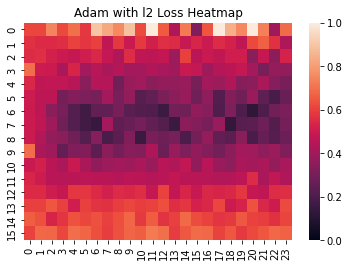
\includegraphics[scale=0.65]{graphs/adam_loss.png}
%             \captionof{figure}{}
%             \label{InVsOutputLen}
%         \end{figure}
%     \end{minipage}
%     \begin{minipage}{0.5 \textwidth}
%         \begin{figure}[H]
%             \centering
%             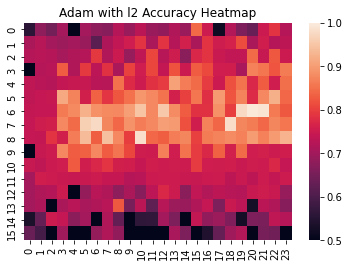
\includegraphics[scale=0.65]{graphs/adam_accuracy.png}
%             \captionof{figure}{}
%             \label{InLenVsRunTime}
%         \end{figure}
%     \end{minipage}

%     \begin{minipage}{0.5 \textwidth}
%         \begin{figure}[H]
%             \centering
%             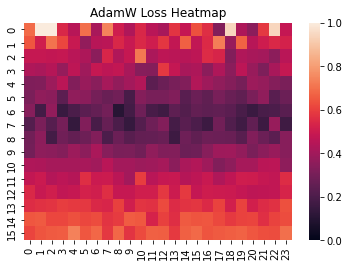
\includegraphics[scale=0.65]{graphs/adamW_loss.png}
%             \captionof{figure}{}
%             \label{InVsOutputLen}
%         \end{figure}
%     \end{minipage}
%     \begin{minipage}{0.5 \textwidth}
%         \begin{figure}[H]
%             \centering
%             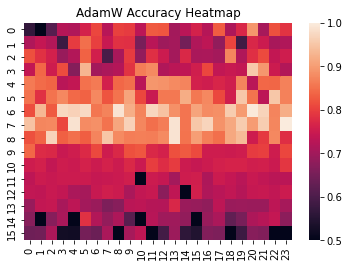
\includegraphics[scale=0.65]{graphs/adamW_accuracy.png}
%             \captionof{figure}{}
%             \label{InLenVsRunTime}
%         \end{figure}
%     \end{minipage}
%     } 

%     \item{
%         Answers will vary, there's simply too many ways to vary the data to account for every answer. In our experimentation, we found typically increasing the difficulty of the data set leads to a larger difference in region of ``good'' hyperparameter combinations between the two algorithms. An easier data set is easier to reach convergence on, and leads to more similar heat maps generated from the two optimizers. Increasing the number of spirals and noise level of the data set are the most effective ways of making the data set ``harder.''
%     }

%     \item{
%         It's very likely the case that for most applications, tuning hyperparameters of AdamW will be easier than tuning hyperparameters of $\ell_2$ regularized Adam. Both models are able to achieve over $99\%$ accuracy over the initially given  settings, but the number of combinations of parameters for AdamW achieving above $90\%$ accuracy is about $50\%$ more than that of $\ell_2$ regularized Adam (raw count from one of our trials are $31$ vs $21$).
%         }
% \end{enumerate}
% }

\end{enumerate}

    
    %\input{problems/(optional)Adam}
    
    % \textbf{(TODO - remove before submission)Grading Rubric}

\textbf{20pt - Working implementation} in a new framework (JAX, Julia, Matlab, or Tensorflow if not used in the original code).
All the code that the students implemented works and is self-contained. Includes instructions for setting up the environment and running without any issues. Solutions do not have bugs and graders are able to run the code without any problems.
Students clearly cite any external sources used (for example, if they used something they found on paperswithcode or a blog post, this is fine, as long as it clearly cited and student have created significant work of their own.) 
Students have clearly made a solid effort and gotten their project in working shape. It doesn’t have to be perfect, and it’s fine if the students have a “wish list” of additional things they would do if they had the time.

\textbf{25pt - Content and Correctness}
Coding questions engage with selected key concepts in the paper and are easy to follow and pedagogically useful. Implementation is doable for someone with CS 182 level mathematical maturity (not too difficult, but not completely trivial either).
Any exposition/mathematical background about the concepts as provided in the problem description is correct. 
Code solutions are provided and fully correct. 
If there are analytical questions, the full LaTeX and PDF export of the assignment (and solutions if separate) are provided. LaTeX files compile correctly. The problems and solutions are completely correct and engage with the material in a pedagogically useful way.
Doing the full problem (coding and written parts) would take an average CS 182 student 1.5-2hr to complete. 


\textbf{15pt - Scaffolding}
Project provides necessary scaffolding for a student to engage with the material. Any code that students are expected to implement is explained clearly through the use of text cells in Jupyter and/or code comments.
If the project group uses any external packages, these are provided, or there are simple instructions on how to download them from before starting the assignment
If possible, autograding tests/sanity checks to make sure a student’s implementation is correct are provided. Gradescope autograder files are not needed—simple sanity checks that compare actual values against expected values are enough. 

\textbf{10pt - Readability/Clarity}
HW assignment and commentary are easy to read and follow. Any mathematical notation used is understandable, and any non-standard notation is clearly explained. The assignment and commentary are free of spelling/grammar errors.



    \newpage
\end{qunlist}

\begin{thebibliography}{00}
    \bibitem{Loshchilov} Loshchilov, Ilya, and Frank Hutter. ‘Decoupled Weight Decay Regularization’. 7th International Conference on Learning Representations, ICLR 2019, New Orleans, LA, USA, May 6-9, 2019. https://arxiv.org/pdf/1711.05101.pdf

%Not used but was helpful
\bibitem{Agarwal} \footnote[1]{\label{note1}These sources were not directly referenced in the paper, but were crucial in understand the concepts better (Adaptive Methods, Adam, etc.) in order to create the problem set.} \hspace{-6mm} Agarwal, Naman \& Bullins, Brian \& Chen, Xinyi \& Hazan, Elad \& Singh, Karan \& Zhang, Cyril \& Zhang, Yi. (2018). The Case for Full-Matrix Adaptive Regularization. https://arxiv.org/pdf/1806.02958.pdf

%Not used but was helpful
\bibitem{Bushaev} \footnotemark[\ref{note1}]Bushaev, Vitaly. (2018). Adam — latest trends in deep learning optimization. https://towardsdatascience.com/adam-latest-trends-in-deep-learning-optimization-6be9a291375c

%Not used but was helpful
\bibitem{Jiang} \footnotemark[\ref{note1}]Jiang, Lili. (2020). A Visual Explanation of Gradient Descent Methods (Momentum, AdaGrad, RMSProp, Adam). https://towardsdatascience.com/a-visual-explanation-of-gradient-descent-methods-momentum-adagrad-rmsprop-adam-f898b102325c

%Not used but was helpful
\bibitem{Villarraga} \footnotemark[\ref{note1}]Villarraga, Daniel. (2021). AdaGrad. https://optimization.cbe.cornell.edu/index.php?title=AdaGrad

\bibitem{Zhang} \footnotemark[\ref{note1}]Zhang, Jiawei. (2019). Gradient Descent based Optimization Algorithms for Deep Learning Models Training. https://arxiv.org/pdf/1903.03614.pdf

\bibitem{ZhangBERT} \footnotemark[\ref{note1}]Zhang, T., Wu, F., Katiyar, A., Weinberger, K., & Artzi, Y.. (2020). Revisiting Few-sample BERT Fine-tuning. https://arxiv.org/pdf/2006.05987.pdf
    % \footnote[1]{These sources were not directly cited in the paper, but were referenced to better understand the concepts (Adaptive Methods, Adam, etc.) and creating the problem set.}
    \newpage
\end{thebibliography}

\end{document}
